\documentclass[10pt,a4paper]{article}
\usepackage[margin=17mm,top=15mm,bottom=16mm]{geometry}
\usepackage[T1]{fontenc}
\usepackage[utf8]{inputenc}
\usepackage{helvet}
\renewcommand{\familydefault}{\sfdefault}
\usepackage{microtype,booktabs,array,tabularx,xcolor,tikz,tcolorbox,fancyhdr,hyperref}
\usetikzlibrary{arrows.meta,positioning,calc}
\definecolor{navy}{HTML}{173653}
\definecolor{teal}{HTML}{087F8C}
\definecolor{pale}{HTML}{EDF6F7}
\definecolor{ink}{HTML}{24374B}
\definecolor{muted}{HTML}{526576}
\definecolor{amber}{HTML}{926316}
\hypersetup{colorlinks=true,urlcolor=teal,linkcolor=teal,pdftitle={Time- and Version-Aware Financial Claim Verification: Supervisor Brief},pdfauthor={B.Tech research project; AI-assisted preparation}}
\pagestyle{fancy}\fancyhf{}\renewcommand{\headrulewidth}{0pt}
\fancyfoot[L]{\scriptsize\color{muted}B.Tech research brief \textbullet\ 27 October 2026 \textbullet\ Provisional research design}
\fancyfoot[R]{\scriptsize\color{muted}\thepage\ / 2}
\setlength{\parindent}{0pt}\setlength{\parskip}{5pt}
\renewcommand{\arraystretch}{1.25}
\newcommand{\sect}[1]{\par\vspace{5pt}{\large\bfseries\color{navy}#1}\par\vspace{1pt}}
\newcommand{\smallhead}[1]{{\bfseries\color{navy}#1}}
\newcommand{\citebrief}[1]{\hyperlink{ref#1}{\textsuperscript{[#1]}}}
\tcbset{colback=pale,colframe=teal!35,boxrule=.5pt,arc=2mm,left=9pt,right=9pt,top=7pt,bottom=7pt}
\begin{document}
\color{ink}
{\scriptsize\bfseries\color{teal}SUPERVISOR BRIEF \quad / \quad ARTIFICIAL INTELLIGENCE + FINANCE}
\vspace{5pt}

{\fontsize{25}{28}\selectfont\bfseries\color{navy}Which financial number\newline counts at which time?}\par
{\large Time- and Version-Aware Financial Claim Verification}

\begin{tcolorbox}
\smallhead{The project in 45 seconds}\par
Companies sometimes correct numbers in their financial reports. A financial AI assistant must therefore check more than whether a number appears in a document: it must use the right report version and the information available at the requested date. We are building a verifier that returns \textbf{supported, contradicted or underdetermined}, with cited evidence. We have a working rule-based prototype and 30 draft pilot cases. Human review is underway; evaluating and integrating existing language models is the next planned stage.
\end{tcolorbox}

\sect{1. The problem, using one real company}
SunPower's fiscal-2022 \textbf{net income attributable to stockholders} changed from \textbf{\$56.037 million} to \textbf{\$42.849 million} in the selected reports. This is a specific statement row, not every measure of the company's income.\citebrief{1}

\begin{center}
\begin{tikzpicture}[>=Latex,node distance=7mm,
 event/.style={draw=teal!45,fill=pale,rounded corners=2mm,text width=4.8cm,minimum height=1.43cm,align=center,inner sep=5pt,font=\small}]
\node[event] (a) {\textbf{10 March 2023}\\Original annual report\\\$56.037 million};
\node[event,right=of a] (b) {\textbf{24 October 2023}\\Non-reliance notice\\Specified old statements\\should not be relied upon};
\node[event,right=of b] (c) {\textbf{18 December 2023}\\Amended annual report\\\$42.849 million};
\draw[->,thick,teal] (a)--(b);\draw[->,thick,teal] (b)--(c);
\end{tikzpicture}
\end{center}
\vspace{-7pt}
{\scriptsize\color{muted}\textbf{Figure 1.} Official filing dates of the selected evidence. Fiscal period: 3 January 2022--1 January 2023.}

\textbf{Claim:} ``SunPower reported stockholder-attributable income of \$56.037 million for fiscal 2022.'' The requested interpretation changes the verdict:

{\small
\begin{tabularx}{\linewidth}{@{}>{\raggedright\arraybackslash}X >{\raggedright\arraybackslash}p{2.8cm} >{\raggedright\arraybackslash}p{6.1cm}@{}}
\toprule
\textbf{What the question asks} & \textbf{Verdict} & \textbf{Why, within this evidence packet}\\\midrule
What did the original report say? & Supported & The original report disclosed that amount.\\
What do the corrected figures say? & Contradicted & The selected corrected amount is \$42.849 million.\\
What did active statements establish on 25 October 2023? & Underdetermined & An eligible withdrawal exists; the selected replacement is still in the future.\\\bottomrule
\end{tabularx}}
{\scriptsize\color{muted}These are provisional interpretations under our explicit evaluation contract. The first two questions use a cutoff after the amendment. ``Underdetermined'' means the supplied evidence cannot settle the claim; it is not automatically a false claim.}

\sect{2. The specific research gap we are investigating}
\textbf{Established prior work:} FinGround says it defaults to the most recent filing when restated figures conflict.\citebrief{2} FinVerBench describes discarding companies with source inconsistencies due to tagging variations or restatements.\citebrief{3}

\textbf{Our proposed focus:} construct and review paired cases that test whether a verifier follows the \emph{requested original/corrected version and historical cutoff}, including a withdrawal before a replacement becomes available. Check the exact metric, period, units and evidence along with the answer.

{\small\color{amber}\textbf{Honest novelty boundary:} this is a literature-motivated candidate gap, not proof of a first-ever method. Temporal checking, financial verification and uncertainty already have prior work. Closest released benchmarks still need fuller inspection.}

\newpage
{\scriptsize\bfseries\color{teal}ENGINEERING PLAN \quad / \quad LLM ROLE, EVALUATION AND CURRENT PROGRESS}
\sect{3. What we will engineer, and where the AI fits}
An \textbf{LLM (large language model)} is a model that reads and generates language. We plan to use existing LLMs to interpret claims and extract evidence from reports. Explicit software checks then enforce the requested dates, versions and numerical consistency. This is the proposed combined system; the present demo starts from prepared facts.

\begin{minipage}[t]{0.49\linewidth}
\vspace{0pt}
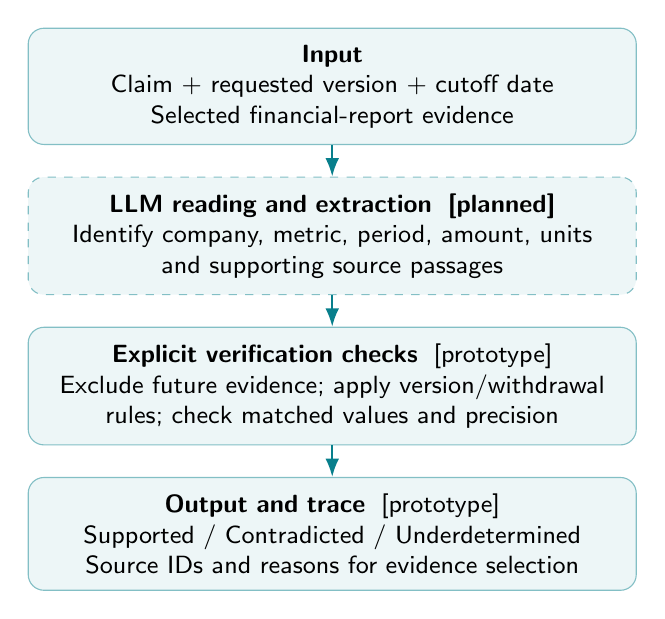
\begin{tikzpicture}[>=Latex,node distance=4mm,
 block/.style={draw=teal!50,fill=pale,rounded corners=2mm,text width=7.3cm,align=center,inner sep=6pt,font=\small},
 future/.style={block,dashed},arr/.style={->,thick,teal}]
\node[block] (input) {\textbf{Input}\\Claim + requested version + cutoff date\\Selected financial-report evidence};
\node[future,below=of input] (llm) {\textbf{LLM reading and extraction \;[planned]}\\Identify company, metric, period, amount, units\\and supporting source passages};
\node[block,below=of llm] (rules) {\textbf{Explicit verification checks}\ \;[prototype]\\Exclude future evidence; apply version/withdrawal\\rules; check matched values and precision};
\node[block,below=of rules] (out) {\textbf{Output and trace}\ \;[prototype]\\Supported / Contradicted / Underdetermined\\Source IDs and reasons for evidence selection};
\draw[arr] (input)--(llm);\draw[arr] (llm)--(rules);\draw[arr] (rules)--(out);
\end{tikzpicture}

{\scriptsize\color{muted}\textbf{Figure 2.} Proposed pipeline. The current demo supplies prepared facts directly to the checks. The dashed stage has not yet been integrated or evaluated.}
\end{minipage}\hfill
\begin{minipage}[t]{0.47\linewidth}
\vspace{1pt}
\smallhead{Why this is an AI engineering project}\par
It combines document understanding, structured evidence extraction, temporal reasoning, a verification engine, a user interface and experimental evaluation in a financial-reporting domain. A useful AI engineering contribution can integrate and evaluate existing models; training a new foundation model is not required.

\vspace{4pt}\smallhead{What the LLM adds}\par
It could reduce manual work in reading filings and interpreting claims. Whether it does so accurately is a \textbf{research question}, not a demonstrated benefit. Its extracted numbers and source links must be checked.

\vspace{4pt}\smallhead{The planned experiment}\par
Compare an \textbf{LLM-only verifier}, a \textbf{strong rule-only control}, and the \textbf{combined system}. Give each the same policy, cutoff and evidence information. Separate tests on prepared evidence from tests on actual source excerpts.

Measure verdict correctness, future-evidence mistakes, source-citation correctness and appropriate uncertainty. Use reviewed labels and report results by issuer; related claims are not independent replications.
\end{minipage}

\sect{4. What is complete, and what comes next}
{\small
\begin{tabularx}{\linewidth}{@{}>{\raggedright\arraybackslash}p{2.1cm} >{\raggedright\arraybackslash}X@{}}
\toprule
\textbf{Status} & \textbf{What we can accurately report}\\\midrule
Implemented & Local browser demo on prepared pilot facts; policy/cutoff controls; verdict and source trace. Eleven software checks passed. These are not accuracy measurements.\\
In progress & 30 draft claims from five issuers and 11 SEC filings. R1 reports reviewing; six calibration cases are prepared. No completed human-review results have been recorded here.\\
Next & Finish calibration and separate student reviews; resolve or exclude ambiguities; freeze a reviewed pilot; correct the LLM evaluation design and run existing models.\\
Not established & Independent model performance, superiority over a strong simple rule, a new algorithm, or publication-level novelty. Broader data screening remains pending.\\\bottomrule
\end{tabularx}}

\textbf{Proposed contribution:} a reviewed evaluation set and an evidence-linked verifier showing when disclosure version and historical availability matter. The current simple withdrawal-aware rule matches the reference resolver on the draft cases; that limits any algorithmic-superiority claim.\citebrief{4}

\textbf{What we need from the supervisor:} agreement on the scope and expected AI implementation depth, feedback on the evaluation design and a review of unresolved cases. Two calibrated students can check explicit filing evidence; difficult accounting interpretations remain unresolved or are excluded. We will not claim expert validation.

\vspace{4pt}\hrule\vspace{3pt}
{\fontsize{7.6}{9.2}\selectfont
\textbf{Selected evidence and references.}\par
\hypertarget{ref1}{[1]} SunPower Corporation. SEC filings: \href{https://www.sec.gov/Archives/edgar/data/867773/000086777323000026/spwr-20230101.htm}{2022 Form 10-K}; \href{https://www.sec.gov/Archives/edgar/data/867773/000086777323000089/spwr-20231018.htm}{24 Oct. 2023 Form 8-K, Item 4.02}; \href{https://www.sec.gov/Archives/edgar/data/867773/000086777323000117/spwr-20230101.htm}{2022 Form 10-K/A, Note 2}. Source packet inspected 26 Oct. 2026; official filing dates and provenance recorded in the pilot.\par
\hypertarget{ref2}{[2]} D. Guo, J. Wu and S. M. Yiu (2026). \emph{FinGround: Detecting and Grounding Financial Hallucinations via Atomic Claim Verification}. \href{https://arxiv.org/html/2604.23588v1}{arXiv:2604.23588v1}, Section 3.3. Preprint; relevant full-text passage rechecked online 27 Oct. 2026.\par
\hypertarget{ref3}{[3]} S. Panda (2026). \emph{FinVerBench: Benchmark Validity and Calibration in Large Language Model Financial Statement Verification}. \href{https://arxiv.org/html/2605.29586v1}{arXiv:2605.29586v1}, data-construction passage. Preprint; relevant full text rechecked online 27 Oct. 2026.\par
\hypertarget{ref4}{[4]} Project records: \href{https://github.com/Shreya732-debug/Research-Work/blob/main/pilot/pilot_assessment.md}{pilot assessment}; \href{https://github.com/Shreya732-debug/Research-Work/tree/main/pilot/calibration}{calibration pack}; \href{https://github.com/Shreya732-debug/Research-Work/tree/codex/supervisor-demo-package/supervisor_demo}{supervisor demo and validation walkthrough}. Internal artifacts, not peer-reviewed findings.
}
\end{document}
